%# -*- coding: utf-8-unix -*-
%%==================================================
%% thesis.tex
%%==================================================

% 双面打印
%\documentclass[doctor, fontset=adobe, openright, twoside, zihao=-4]{sjtuthesis}
 \documentclass[bachelor, fontset=adobe, openany, oneside, zihao=-4]{sjtuthesis} 
% \documentclass[master, adobefonts, review]{sjtuthesis} 
% \documentclass[%
%   bachelor|master|doctor,	% 必选项
%   fontset=adobe|windows,  	% 只测试了adobe
%   oneside|twoside,		% 单面打印,双面打印(奇偶页交换页边距,默认)
%   openany|openright, 		% 可以在奇数或者偶数页开新章|只在奇数页开新章(默认)
%   zihao=-4|5,, 		% 正文字号:小四、五号(默认)
%   review,	 		% 盲审论文,隐去作者姓名、学号、导师姓名、致谢、发表论文和参与的项目
%   submit			% 定稿提交的论文,插入签名扫描版的原创性声明、授权声明 
% ]

\begin{document}

%% 无编号内容:中英文论文封面、授权页
%# -*- coding: utf-8-unix -*-
\title{基于多模态深度自编码器情绪识别研究}
\author{付\quad{}豪}
\advisor{吕宝粮教授}
% \coadvisor{某某教授}
\defenddate{2016年6月14日}
\school{上海交通大学}
\institute{计算机科学与工程系}
\studentnumber{5120309235}
\major{计算机科学与工程}

\englishtitle{Multi-modal Deep Auto-encoder Based Emotion Recognition}
\englishauthor{\textsc{Hao Fu}}
\englishadvisor{Prof. \textsc{Bao-liang Lu}}
% \englishcoadvisor{Prof. \textsc{Uom Uom}}
\englishschool{Shanghai Jiao Tong University}
\englishinstitute{\textsc{Depart of Computer Science and Engineering, School of SEIEE} \\
  \textsc{Shanghai Jiao Tong University} \\
  \textsc{Shanghai, P.R.China}}
\englishmajor{Computer Science and Engineering}
\englishdate{Jun. 14th, 2016}


\maketitle

\makeenglishtitle

\makeatletter
\ifsjtu@submit\relax
	\includepdf{pdf/original.pdf}
	\cleardoublepage
	\includepdf{pdf/authorization.pdf}
	\cleardoublepage
\else
	\makeDeclareOriginal
	\makeDeclareAuthorization	
\fi
\makeatother


\frontmatter 	% 使用罗马数字对前言编号

%% 摘要
\pagestyle{plain}
%# -*- coding: utf-8-unix -*-
%%==================================================
%% abstract.tex for SJTU Master Thesis
%%==================================================

\begin{abstract}
随着计算机的发展,我们期望能用一种高效而且准确的方法识别人类的情绪,从而在人机交互与人人交互中发挥巨大的作用。在基于各种信号的情绪识别中,基于脑电信号的情绪识别算法由于与激发情绪的大脑活动有直接关联,无疑成为当前最有可能获得较高准确度的情绪识别算法之一。因此,建立一套能广泛适用于不同个体之间的算法模型有着非常重要的实际意义,也成为当下基于脑电信号的情绪识别研究的热点之一。与此同时,随着机器的计算能力的提高,深度学习的方法例如卷积神经网络,深度置信网络,深度自编码器等受到研究人员的青睐。但是如果只是用单一模态的输入进行学习,由于数据的分布总是相似的,所以提供的信息和学习能力都是很有限的。相反,不同模态譬如声音,文字,图像,脑电,眼动轨迹带有不同信息,所以提供的数据分布各不相同,他们各自提供的信息不但有交集,还互相补充。因此,如果能够利用多模态输入信号的融合,我们不仅可以提取出多模态共有的特征表达,从而找出它们代表的现实世界中的意义,还可以利用多个模态不同信号的互补信息来提高情绪识别任务的准确率。

\keywords{\large 深度学习 \quad 深度自编码器 \quad 多模态 \quad 互补特征}
\end{abstract}

\begin{englishabstract}

	With the development of computers, we can expect an efficient and accurate method of identifying human emotions, which play a huge role in human-computer interaction and human interaction in. In the emotion recognition based on various signals, emotion recognition algorithm based on brain electrical signal due to excitation emotional brain activity directly related, it will undoubtedly become one of the most likely to get the emotion recognition algorithm high accuracy. Therefore, the establishment of a widely applicable model algorithm has a very important practical significance between different individuals, it has become one of the hot emotion recognition based on the current EEG. In the meantime, with the improvement of the machine's computing power, depth of learning methods such as convolution neural network, the depth of belief networks, since the depth encoder favored by researchers. However, if only a single mode input learning, since the distribution of the data is always similar, so the ability to provide information and learning are very limited. Instead, different modalities such as voice, text, image, EEG, eye movement trajectory with different information, so the data provided by each of the distribution are not identical, they each provide information not only joy, but also complement each other. Therefore, if harnessed fusion multimodal input signal, we can extract only feature common to multi-modal expression, to find out the real world in the sense that they represent can also use complementary information of a plurality of signals of different modes to improve the accuracy of emotion recognition task.
	
\englishkeywords{\large Deep learning \quad Deep auto-encoder \quad multi-modal \quad feature-complement}
\end{englishabstract}



%% 目录、插图目录、表格目录
\tableofcontents
\listoffigures
\addcontentsline{toc}{chapter}{\listfigurename} %将插图目录加入全文目录
\listoftables
\addcontentsline{toc}{chapter}{\listtablename}  %将表格目录加入全文目录
% \listofalgorithms
% \addcontentsline{toc}{chapter}{算法索引}        %将算法目录加入全文目录

%# -*- coding: utf-8-unix -*-
\chapter{主要符号对照表}
\label{chap:symb}

\begin{longtable}{rl}
$\epsilon$     & 介电常数 \\
 $\mu$ 		& 磁导率 \\
 $\epsilon$     & 介电常数 \\
 $\mu$ 		& 磁导率 \\
 $\epsilon$     & 介电常数 \\
 $\mu$ 		& 磁导率 \\
 $\epsilon$ 	& 介电常数 \\
 $\mu$ 		& 磁导率 \\
 $\epsilon$     & 介电常数 \\
 $\mu$ 		& 磁导率 \\
 $\epsilon$     & 介电常数 \\
 $\mu$ 		& 磁导率 \\
 $\epsilon$     & 介电常数 \\
 $\mu$ 		& 磁导率 \\
 $\epsilon$ 	& 介电常数 \\
 $\mu$ 		& 磁导率 \\
 $\epsilon$     & 介电常数 \\
 $\mu$ 		& 磁导率 \\
 $\epsilon$     & 介电常数 \\
 $\mu$ 		& 磁导率 \\
 $\epsilon$     & 介电常数 \\
 $\mu$ 		& 磁导率 \\
 $\epsilon$ 	& 介电常数 \\
 $\mu$ 		& 磁导率 \\
 $\epsilon$     & 介电常数 \\
 $\mu$ 		& 磁导率 \\
 $\epsilon$     & 介电常数 \\
 $\mu$ 		& 磁导率 \\
 $\epsilon$     & 介电常数 \\
 $\mu$ 		& 磁导率 \\
 $\epsilon$ 	& 介电常数 \\
 $\mu$ 		& 磁导率 \\
 $\epsilon$     & 介电常数 \\
 $\mu$ 		& 磁导率 \\
 $\epsilon$     & 介电常数 \\
 $\mu$ 		& 磁导率 \\
 $\epsilon$     & 介电常数 \\
 $\mu$ 		& 磁导率 \\
 $\epsilon$ 	& 介电常数 \\
 $\mu$ 		& 磁导率 \\
 $\epsilon$     & 介电常数 \\
 $\mu$ 		& 磁导率 \\
 $\epsilon$     & 介电常数 \\
 $\mu$ 		& 磁导率 \\
 $\epsilon$     & 介电常数 \\
 $\mu$ 		& 磁导率 \\
 $\epsilon$ 	& 介电常数 \\
 $\mu$ 		& 磁导率 \\
 $\epsilon$     & 介电常数 \\
 $\mu$ 		& 磁导率 \\
 $\epsilon$     & 介电常数 \\
 $\mu$ 		& 磁导率 \\
 $\epsilon$     & 介电常数 \\
 $\mu$ 		& 磁导率 \\
\end{longtable}
 % 主要符号、缩略词对照表

\mainmatter	% 使用阿拉伯数字对正文编号

%% 正文内容
\pagestyle{main}
%# -*- coding: utf-8-unix -*-
%%==================================================
%% chapter01.tex for SJTU Master Thesis
%%==================================================

%\bibliographystyle{sjtu2}%[此处用于每章都生产参考文献]
\chapter{绪论}
\label{chap:intro}
	一直以来,情绪都被认为是高级生命体独有的特征。而它是极其复杂的心理现象,是一种多成分、多维度、多种类组合的心理过程。每个人的情绪不但与自己的认知息息相关,每种情绪还可以相互组合从而派生出更复杂而高级的情绪。心理现象是脑的功能,所以大脑是产生不同情绪的根源所在,所以基于脑电信号的情绪识别方法无疑最可能成为有最高准确率的方法之一。因此,建立一套准确,方便同时广泛适用的模型对于情绪的研究来说意义重大。此时,基于脑电信号分析的算法可以发挥效用。


\section{研究背景与意义}

	每个人无时无刻都不在产生情绪,情绪在日常生活中时刻都在陪伴着我们,它不但影响着我们的一举一动,还会对我们的健康产生积极或者消极的影响。积极的情绪可以带给人民愉悦感,获得好的心情并且提高工作效率。并且有科学证据表明,愉快喜悦等积极情绪还可以使得伤口加快愈合,促进疾病痊愈。与此相反,消极的情绪会阻碍人们的个性发展,降低人们的自信和自我评价,还会影响人们的认知思维水平,妨碍日常生活。长期生活在抑郁、忧郁或恐惧下的人或性格古怪,社交能力较差,从而影响他们的生活质量。
	情绪可以有多种方式被表达,譬如语言文字,肢体语言,面部表情等等。但是与脑电图(Electroencephalograph, 简称:EEG)信号相比,提供的数据有特征不突出,没有明显的模式的特点,加大了我们使用这些数据的难度,所以利用EEG信号来识别情绪可以获得比较好的准确率。而这项研究也成为当今EEG领域的热点之一。
	EEG 信号是由电极采集在人体脑部自身产生的微弱生物电,然后在头皮处经放大后而得到数据。 这种信号最初是用于癫痫、脑血管疾病的检查,而现在由于它的时效性和前文所述的多种优点, 已经在多个领域被广泛利用,包括情绪识别,医疗,虚拟现实等等。而利用脑电信号来进行情绪识别的最大优点就是可以在保持识别过程的迅速的基础上,有更好的准确率,为进一步的各个细分领域的研究打下了坚实的基础。举例来说,譬如帮助抑郁症患者或者受到重大精神打击的人进行情绪分析,从而让医生了解病人真正的情绪,提供更好的治疗方案。或者对正在执行任务的警察保持情绪的观察,如果出现不正常的愤怒等情绪可以利用合适的方法来提醒。或者在远程教育方面,实时地情绪识别可以帮助老师快速地了解学生们的情绪状态,并以此为依据来在课上调整授课内容与方式, 保证教学的质量和灵活性。
	与此同时,随着机器的计算能力的提高,深度学习的方法例如深度置信网络,深度自编码器等受到研究人员的青睐。但是如果只是用单一模态的输入进行学习,由于数据的分布总是相似的,所以提供的信息和学习能力都是很有限的。相反,不同模态譬如声音,文字,图像,脑电,眼动轨迹带有不同信息,所以提供的数据分布各不相同,他们各自提供的信息不但有交集,还互相补充。因此,如果能够利用多模态输入信号的融合,我们不仅可以提取出多模态共有的特征表达,从而找出它们代表的现实世界中的意义,还可以利用多个模态不同信号的互补信息来提高情绪识别任务的准确率。
	所以,本课题的目标在于把眼动轨迹和EEG信号进行融合,找到合适且快速的融合方法,从而利用多模态的信息来进行情绪识别,这样就可以利用眼动轨迹和EEG信号所能提供的互补信息来获得比只是利用单一模态信息更好的表现。
	
\section{国内外研究现状}
	 N Srivastava[1]利用多模态Deep Boltzmann Machines(DBM),作为模型,对图像和文字进行了多模态深度学习。获得了比深度自编码器和多模态DBN更好的结果。 利用多模态DBM学习得共同特征作为输入也在单模态学习中超过了原始的文字模态作为输入。
	Ngiam et al. [2] 用深度自编码器进行了语音和视频的多模态深度学习。他们分别利用了只有声音一个模态和声音和视频两个模态作为输入,利用RBM重建声音和视频两个模态的特征并寻找共同表达。最终结论为,用声音一个模态作为输入,而两个RBM分别重建声音和视频的特征寻找到的共同特征表达有最好的结果。
	Xing et al. [3] 用dual-wing harmoniums的模型进行了文字和图像的多模态深度学习,他们使用了包含高斯隐含单元,高斯和泊松可见单元的线性RBM模型,最终结果明显好Gaussian-multinomial mixture 和 Gaussian-multinomial mixture LDA.
	 
	 
\section{工作介绍}
	本课题将着重研究如何将实验室获得的眼动仪数据和EEG信号相融合,使得利用两个模态作为输入信息的算法模型有相比于单纯利用EEG信号或者眼动仪数据的算法有更好的表现。目前国内外对语基于脑电信号的情绪研究和多模态学习分别都有深入的研究,但是将多模态学习利用在情绪识别,特别是在EEG信号的利用上还远远不足。
	我们通过对脑电信号和眼动仪信号的分析,对十一个被试人,每个人三组共三十三组的数据进行处理。结合多模态学习在其他领域的方法,提出了我们的多模态深度学习的算法模型,并且最终使得情绪识别的准确率有所提升。
\section{本章小结}
	本章主要介绍了基于多模态深度学习的情绪识别研究的目的和意义,以及多模态学习,脑电 情绪研究在国内外的研究现状。
%# -*- coding: utf-8-unix -*-
%%==================================================
%% chapter02.tex for SJTU Master Thesis
%%==================================================

%\bibliographystyle{sjtu2}%[此处用于每章都生产参考文献]
\chapter{情绪及情绪刺激}
\label{chap:chap2}
	


\section{情绪定义}
情绪在心理学上的定义是:人们对需求和客观事物两者关系的应激性反应,是一种每个人不同的主观感受、也是每个人都有的生理反应、还是认知的互动,并且有表达出特定的行为的趋势。同时,也有很多相关学者认为情绪和认知联系紧密,不可分割。另外,情绪表达与情绪不同,前者是一个人的内在情绪通过表情、动作、语言等方式表现出来。在意识和价值观的作用下,每个人所表达的情绪可能是强化或者弱化的真正的情绪。我们可以总结出以下几点:
\begin{itemize}
  \item 情绪是本身对外界的一种自然反应。情绪没有好坏对错,而是一种离散的对外界或者内部的刺激而自然产生的反应。
  \item 情绪是外来刺激和内在认知的一种互动。正面或负面情绪的出现,分别是自身对需求得到满足和未得到满足时产生的生理反应。这也就是情绪的生理特征。
  \item 情绪有情绪表达的趋势。情绪是由外而内的感受和刺激带来的,然后又由内而外的表达。这也就是情绪的表达和动作趋势。
\end{itemize}

\section{情绪理论}
	\centerline{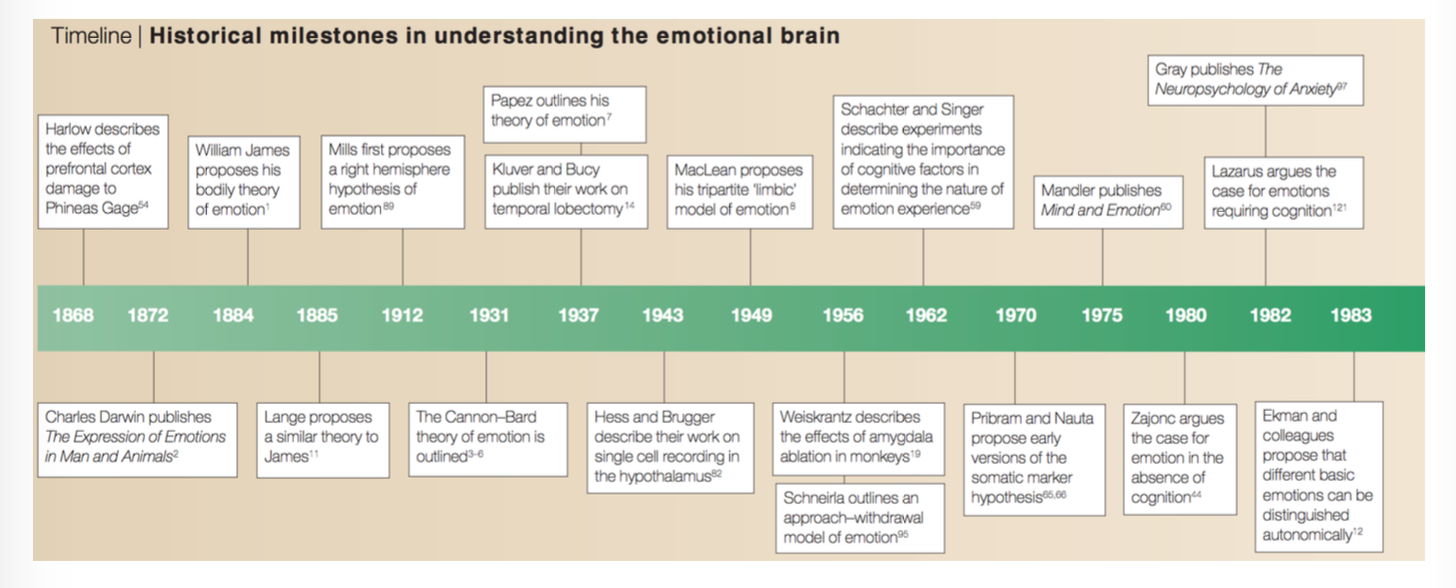
\includegraphics[width=5in]{figure/timeline.png}}
	本节将列举几个广泛使用的情绪模型:
	\begin{itemize}
		\item James Lange理论。这是发表于1884年的一篇论文,并且首次给出了情绪的定义。这个理论认为身体对外部事件产生的生理反应的结果就是情绪,是由生理学派首创的十分著名的理论。
		\item Cannon Bard理论。这个理论否定了上条理论,他们通过试验,发现无论有没有身体的响应,大脑都会产生情绪。因此,他们认为当来自外界的刺激传入到大脑之后,丘脑和大脑皮层就会被激活,从而产生了情绪。这个理论肯定了丘脑的关键作用,但是完全否定了身体和情绪的联系,这是它的不足之处。
		\item Schachter Singer理论。这个理论认为人们会对自己正在经历的情绪而产生相应的生理反应,并且注重外界环境对这种生理反应的解释。举例来说,譬如一个人在奔跑,如果是遇到了危险而逃命,那么这个理论将情绪解释为害怕;而如果是一个人跑向他喜欢的人,那么可以将这个情绪解释为激动。
		\item Opponent Process理论。不同于上述所有,这个理论从对比和对立的角度解释情绪的产生。每个人的基本情绪都有对立的情绪,当某种情绪特别突出,压过了它的对立部分,那么我们就认为自己产生了这个情绪。这个理论十分适合解释吸毒成瘾,吸毒上瘾者为了不断体验到毒品带来的感受,就会不断的吸毒,并且越来越严重。
		\item Papez Maclean理论。 Papez提出了环路理论,解释了整个情绪产生的通路,也就是从外部的刺激到产生情绪信号的大脑内部的整个通路。 Maclean在这个基础上又提出了内脏脑,它的职能是调节与情绪相关的组织和器官,并且通过丘脑调节内脏和骨骼的相应反应。
	\end{itemize}
\section{情绪分类与情绪分类模型}
	一直以来,都有两种不同的观点来进行情绪的度量。一种认为情绪是离散并且是可以相互叠加从而派生出新的情绪的。另一种是认为情绪是连续的并且可以进行测量,他们之间只有强度的差别。本论文的基本观点是情绪可以分成多个类别的。
	\centerline{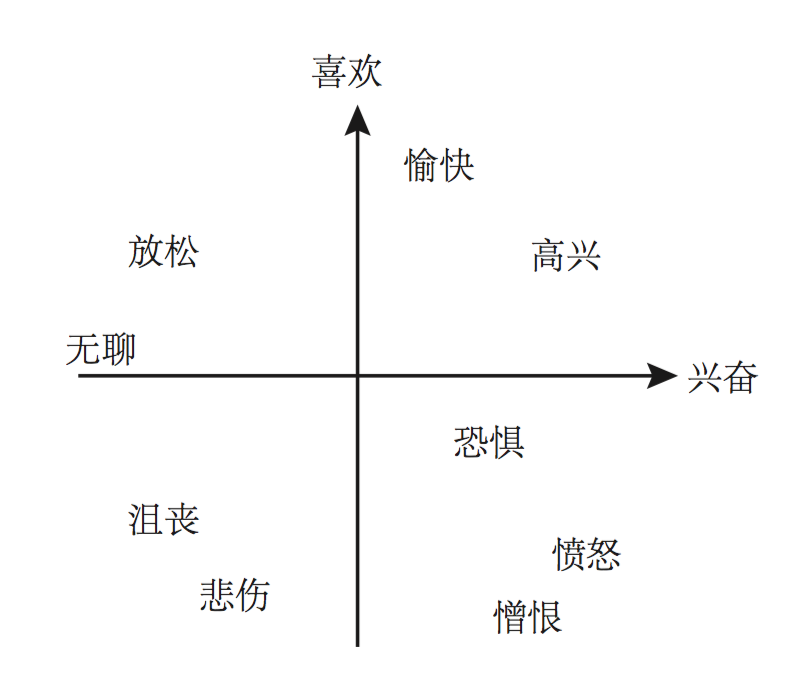
\includegraphics[width=3.5in]{figure/emotion.png}}
	 \subsection{基本情绪}
	 P. Ekman提出的理论认为情绪是离散可叠加并且可以独立的被测量。他最有影响力的研究成果是有六类基本情绪是跨越了种族和国界而广泛适用于人类中的,基于他的研究成果,他提出论点认为人的情绪需要分成六种:愤怒,悲伤,高兴,恐惧,厌恶和惊愕。 而James的情绪集合却包括了愤怒,恐惧,悲伤等\upcite{emotion}。Clynes的情绪集合包括了愤怒,厌恶,悲哀,快乐,浪漫,仇恨,中性等等。Izard的情绪集合包括了愤怒,悲伤,害怕,关心,内疚,快乐等等。
	 
	 不但情绪的划分如此众口不一,我们还很难找到明确的标尺去区别不同的情绪。随着这些年科研工作者的努力,我们才渐渐可以得知不同情绪之间的联系。譬如愤怒的情绪可以转变成为悲伤的情绪。为了让这种关联可视化,我们采用Lange的情绪分类模型,见上图。纵坐标表示的是人们的愉悦度,从厌恶到喜欢。横坐标表示兴奋程度,从低迷到兴奋。这样一来,多种不同的情绪就可以分解开来,通过这个两维度的坐标系显示出来。
	 
	 特别地,J. Panksepp在上世纪提出了大脑中情绪的定义,给出了四种最基本的情绪系统,并且认为这是四种动物出生后不久就拥有的。
	 \begin{itemize}
	 	\item 寻找。 寻找的情绪让情绪的产生者对认识世界充满了好奇,并且进行目的驱动下的寻找,从而找到生存的环境和物品,生存下去。
		\item 害怕。害怕的情绪对疼痛等外界刺激做出反应,害怕情绪的产生会造成战斗,逃遁或者颤栗的行为。
		\item 愤怒。愤怒的情绪通常由于沮丧,外部刺激,身体自由的限制等等引起。
		\item 恐慌。恐慌的情绪通常用于和母亲的分离而引起,它会造成哭泣,叫喊等等行为。
	 \end{itemize}
	 \subsection{多维度情绪表示}
	 利用数据可视化的原理,我们可以在二维模型上将所有情绪描述出来。自然地,相似的情绪状态在二维坐标系中应该距离更近,而相差愈大的情绪状态在坐标系中应该距离更远。通常,心理学家们把这两个用于可视化情绪的维度分别叫做警觉度和效价。后者主要表示情绪的消极/积极程度,而前者代表情绪给人带来刺激的强度。可以用下图(图2-1)表示。
	 \subsection{情绪}
	 虽然在每天平淡的生活中,每个人无时无刻都不被感情充斥着,但是感情却很难完全由自己控制。因此,在实验搜集数据时,我们对能够快速调动并激发实验参与者某些特定情绪和感情的方法有迫切的需求,并且要有较好的可依赖性,鲁棒性和可持续性。在观察了现有研究者尝试过的多种方法以后,论文决定采用视频库作为被试者观看的素材,也就是刺激材料。
	 通过广泛的搜索,本文作者找到了大量汉语作为音频的国内外电影或微电影,排除对英语接受程度不同这个额外变量的影响。不同于P. Ekman提出的六种基本情绪的分类,本文选取高兴,悲伤,中性三种区别最为显著的基本兴趣。在数据收集阶段,实验室通过询问大量与实验参与者各方面条件都类似的学生的评价,根据评价的高低最终选出了15段视频片段作为最终的实验素材。
	 最后,为了保证数据的可信程度和获取足够数量的数据,每个被试都分别进行三次的实验。这也为我们下一步继续研究基于个体的情绪识别研究提供了数据。
\section{本章小结}
	本章对情绪的定义,种类,分类的不同方式和情绪的二维可视化方法做了基本介绍。基于上述的情绪评价模型,本文针对相关需求使用了特定的素材,最终采集到了适合进行EEG和眼动仪信号多模态分析的数据。


%# -*- coding: utf-8-unix -*-
%%==================================================
%% chapter02.tex for SJTU Master Thesis
%%==================================================

%\bibliographystyle{sjtu2}%[此处用于每章都生产参考文献]
\chapter{数据预处理}
\label{chap:chap3}

\section{脑电信号数据预处理流程}
	在本论文中,在进行多模态深度学习之前,需要先将提取到的脑电原始数据进行预处理,而从原始数据转化到我们的输入数据需要经过三个步骤:消除噪声去除伪迹,特征提取和特征平滑。详细流程图请见下图:\\
	由于脑电十分微弱($\mu$V级),采集EEG信号过程中受到的干扰非常多,因此我们拿到的原始数据并不是纯粹的脑电数据,而在其中夹杂了很多噪音。为了解决这个问题,我们应该首先对原始数据进行合适的预处理,在保留有用的EEG信号的前提下,删除掉夹杂着的噪音信号。另外,由于同一个视频片段的情绪应该是一定的,不会出现突然由令人高兴到令人悲伤的跌宕起伏的情节,所以情绪的变化理应稳定平滑,不应该出现剧烈的改变。因此我们认为EEG信号的剧烈变化是由于非情绪相关的大脑其他活动引起的,譬如回忆。所以,我们同样有必要对数据进行平滑处理,这样就可以消除脑电信号的剧烈抖动,增加信号的稳定性和数据的可信度。
\section{消除噪声和去伪迹}
	由于上述原因,我们总结出了以下几种干扰,都是由非情绪相关的大脑活动产生的。
	\begin{itemize}
	\item 眼电伪迹:大脑发出控制眼球的指令就会产生电流,从而形成这种与情绪无关的脑电信号,对于我们的原始数据而言,它是需要去除的噪声。频率为1-50Hz.
	\item 肌电伪迹:由于人不可能保持完全静止的状态,所以肌肉的运动会产生脑电信号,对比于反应情绪的微弱脑电信号,肌电信号可以达到相当大,产生很大程度的污染,大大影响我们提出的数据。
	\item 心电伪迹:心跳的过程也会产生电场和脑电信号,作为我们数据的噪声,频率大约在1Hz。
	\item 皮电干扰:由于人的排汗和空气湿度变化,涂抹在脑电电极周围的脑电膏会产生一定程度的浓度改变等,影响脑电信号的稳定性,从而产生了噪声。
	\end{itemize}
	
	我们首先对原始数据进行降采样,采样率为200Hz。另外,由于1-50Hz的脑电信号是具有明确生理意义的,所以我们才去原始数据以后先进行滤波,提取出1-75Hz的信号,这一步即可消除大部分噪声。

\section{脑电特征提取}
	原始数据经过降采样之后依旧是在时域上,为了保持与之前实验室成果的对比,以及利用EEG信号在频域上的生理意义,本论文采用EEG的频域特征作为输入特征,并分析其与情绪的关系。
	\subsection{时域到频域的特征变换}
		在这个步骤中,离散短时傅立叶变换(Short-Term Fourier Transform, 简称为STFT)是常用并且快速有效的方法。
		
		如果我们设$x[n] = {x_1,…, x_n}$为某一电极上,每个时间窗采集到的原始数据样本数。那么我们就可以利用STFT算法得到下式:
		\begin{align}
		STFT{X[n]}(m, \omega_{k}) \heartsuit X(m, \omega_{k}) = \sum_{n = 1}^N x[n]w[n-m]e^{-j\omega_k n}
		\end{align}
		
	其中,k为整数,并且定义区间是[0,N), $\omega_k = \frac{2\pi k}{N}$,并且w是一个窗口函数,它的作用是对每一个窗口独立地进行傅立叶变换,当我们把整个信号按照时序分成很多片段然后每个片段分别进行傅立叶变换,那么就得到了每个窗口所代表时间的频域信号。这样既得到了频域信息,又没有在整个时域直接进行变换,从而保留了部分时序性,减少了原始信号的时间方面的信息丢失,也为之后对循环神经网络等需要时间信息输入的研究提供了数据。
	
	汉宁窗是常见的窗口函数,也是本论文所使用的。定义如下:
	\begin{align}
	 w[n]=\left\{
	\begin{aligned}
	x & = 0.5[1-\cos(\frac{2\pi n}{M - 1})] ,  & 1 \leq n < M\\
	0 &, & otherwise \\
	\end{aligned}
	\right.
	\end{align}
	
	经过多次试验和测试,我们决定采用窗口大小为4秒的汉宁窗函数。
	
	现在的研究有充分的证据证明,1-50Hz频段的脑电信号有明确生理意义,它被更细的划分为代表1-4Hz的Delta频段, 4-8Hz的Theta频段,8-13Hz的Alpha频段,13-30Hz的beta频段和30-50Hz的Gamma频段。我们首先利用傅立叶变换得到每个频段的信号,然后再利用傅立叶变换计算的到每个频段的能谱:
	\begin{align}
	E(\omega_k) = X(m, \omega_k) * X^*(m, \omega_k)
	\end{align}
	其中*代表的是共轭函数的意思。
	
	经过傅立叶变换和后续计算以后,我们得到的EEG信号有62个频道,而每个频道可以分成5个更细的频段,所以我们最终的特征就是310维的向量,也就是我们深度学习网络的输入向量。
	\subsection{微分熵特征}
	微分熵(英文Differential Entropy,简称DE)由香农熵拓展而来,它描述随机变量的熵。
	设随机变量X,则X的概率密度函数$p(x)$的支持为集合C.那么它的微分熵$h(X)$可以由下式表示:
	\begin{align}
	h(X) = -\int_C f(x)logf(x)dx
	\end{align}
	自然地,我们可以用高斯分布来作为脑电信号的分布的假设,如此便可获得脑电信号离散序列的微分熵如下:
	\begin{align}
	h(X) &=  -\int_{\infty}^{-\infty} {\frac{1}{\sqrt{2\pi \sigma^2}} e^{\frac{{(x-\mu)}^2}{2\sigma^2}}log(\frac{1}{\sqrt{2\pi \sigma^2}}e^{\frac{{(x-\mu)}^2}{2\sigma^2}})dx} \\
	&=\frac{log(2\pi e \sigma^2)}{2}
	\end{align}
	通过对式(3-6)的分析,我们可以看出EEG信号的DE特征只与$\sigma^2$有关,同时,在去除了平均值以后,我们可以通过下式得出EEG信号的方差:
	\begin{align}
	\sigma^2 = \frac{1}{N} \sum_{i=1}^{N}{{x_i}^2}
	\end{align}
	根据式(3-7)我们可以看出方差$\sigma^2$与能量$P_i$是正比关系,因此再根据式(3-6)可得下式:
	\begin{align}
	h_i(X) = \frac{1}{2}log(2\pi e \sigma_i^2) = \frac{1}{2}log P_i + \frac{1}{2}log(\frac{2\pi e}{N})
	\end{align}
	经过进一步简化,我们可以得到下式:\\
	\begin{align}
	h_i(X) = log P_i
	\end{align}
	
%# -*- coding: utf-8-unix -*-
%%==================================================
%% chapter02.tex for SJTU Master Thesis
%% based on CASthesis
%% modified by wei.jianwen@gmail.com
%% Encoding: UTF-8
%%==================================================

\chapter{ \LaTeX 排版例子}
\label{chap:example}

\section{列表环境}
\label{sec:list}

\subsection{无序列表}
\label{sec:unorderlist}

以下是一个无序列表的例子,列表的每个条目单独分段。

\begin{itemize}
  \item 这是一个无序列表。
  \item 这是一个无序列表。
  \item 这是一个无序列表。
\end{itemize}

使用\verb+itemize*+环境可以创建行内无序列表。
\begin{itemize*}
  \item 这是一个无序列表。
  \item 这是一个无序列表。
  \item 这是一个无序列表。
\end{itemize*}
行内无序列表条目不单独分段,所有内容直接插入在原文的段落中。

\subsection{有序列表}
\label{sec:orderlist}

使用环境\verb+enumerate+和\verb+enumerate*+创建有序列表,
使用方法无序列表类似。

\begin{enumerate}
  \item 这是一个有序列表。
  \item 这是一个有序列表。
  \item 这是一个有序列表。
\end{enumerate}

使用\verb+enumerate*+环境可以创建行内有序列表。
\begin{enumerate*}
  \item 这是一个默认有序列表。
  \item 这是一个默认有序列表。
  \item 这是一个默认有序列表。
\end{enumerate*}
行内有序列表条目不单独分段,所有内容直接插入在原文的段落中。

\subsection{描述型列表}

使用环境\verb+description+可创建带有主题词的列表,条目语法是\verb+\item[主题] 内容+。
\begin{description}
    \item[主题一] 详细内容
    \item[主题二] 详细内容
    \item[主题三] 详细内容 \ldots
\end{description}

\subsection{自定义列表样式}

可以使用\verb+label+参数控制列表的样式,
详细可以参考WikiBooks\footnote{\url{https://en.wikibooks.org/wiki/LaTeX/List_Structures\#Customizing_lists}}。
比如一个自定义样式的行内有序列表
\begin{enumerate*}[label=\itshape\alph*)\upshape]
  \item 这是一个自定义样式有序列表。
  \item 这是一个自定义样式有序列表。
  \item 这是一个自定义样式有序列表。
\end{enumerate*}

\section{数学排版}
\label{sec:matheq}

\subsection{公式排版}
\label{sec:eqformat}

这里有举一个长公式排版的例子,来自\href{http://www.tex.ac.uk/tex-archive/info/math/voss/mathmode/Mathmode.pdf}{《Math mode》}:

\begin {multline}
  \frac {1}{2}\Delta (f_{ij}f^{ij})=
  2\left (\sum _{i<j}\chi _{ij}(\sigma _{i}-
    \sigma _{j}) ^{2}+ f^{ij}\nabla _{j}\nabla _{i}(\Delta f)+\right .\\
  \left .+\nabla _{k}f_{ij}\nabla ^{k}f^{ij}+
    f^{ij}f^{k}\left [2\nabla _{i}R_{jk}-
      \nabla _{k}R_{ij}\right ]\vphantom {\sum _{i<j}}\right )
\end{multline}

\subsection{SI单位}

使用\verb+siunitx+宏包可以方便地输入SI单位制单位,例如\verb+\SI{5}{\um}+可以得到\SI{5}{\um}。

\subsubsection{一个四级标题}
\label{sec:depth4}

这是全文唯一的一个四级标题。在这部分中将演示了mathtools宏包中可伸长符号(箭头、等号的例子)的例子。

\begin{displaymath}
    A \xleftarrow[n=0]{} B \xrightarrow[LongLongLongLong]{n>0} C 
\end{displaymath}

\begin{eqnarray}
  f(x) & \xleftrightarrow[]{A=B}  & B \\
  & \xleftharpoondown[below]{above} & B \nonumber \\
  & \xLeftrightarrow[below]{above} & B
\end{eqnarray}

又如:

\begin{align}
  \label{eq:none}
  & I(X_3;X_4)-I(X_3;X_4\mid{}X_1)-I(X_3;X_4\mid{}X_2) \nonumber \\
  = & [I(X_3;X_4)-I(X_3;X_4\mid{}X_1)]-I(X_3;X_4\mid{}\tilde{X}_2) \\
  = & I(X_1;X_3;X_4)-I(X_3;X_4\mid{}\tilde{X}_2)
\end{align}

\subsection{定理环境}

模板中定义了丰富的定理环境
algo(算法),thm(定理),lem(引理),prop(命题),cor(推论),defn(定义),conj(猜想),exmp(例),rem(注),case(情形),
bthm(断言定理),blem(断言引理),bprop(断言命题),bcor(断言推论)。
amsmath还提供了一个proof(证明)的环境。
这里举一个“定理”和“证明”的例子。
\begin{thm}[留数定理]
\label{thm:res}
  假设$U$是复平面上的一个单连通开子集,$a_1,\ldots,a_n$是复平面上有限个点,$f$是定义在$U\backslash \{a_1,\ldots,a_n\}$上的全纯函数,
  如果$\gamma$是一条把$a_1,\ldots,a_n$包围起来的可求长曲线,但不经过任何一个$a_k$,并且其起点与终点重合,那么:

  \begin{equation}
    \label{eq:res}
    \ointop_{\gamma}f(z)\,\mathrm{d}z = 2\uppi\mathbf{i}\sum^n_{k=1}\mathrm{I}(\gamma,a_k)\mathrm{Res}(f,a_k)
  \end{equation}

  如果$\gamma$是若尔当曲线,那么$\mathrm{I}(\gamma, a_k)=1$,因此:

  \begin{equation}
    \label{eq:resthm}
    \ointop_{\gamma}f(z)\,\mathrm{d}z = 2\uppi\mathbf{i}\sum^n_{k=1}\mathrm{Res}(f,a_k)
  \end{equation}

      % \oint_\gamma f(z)\, dz = 2\pi i \sum_{k=1}^n \mathrm{Res}(f, a_k ). 

  在这里,$\mathrm{Res}(f, a_k)$表示$f$在点$a_k$的留数,$\mathrm{I}(\gamma,a_k)$表示$\gamma$关于点$a_k$的卷绕数。
  卷绕数是一个整数,它描述了曲线$\gamma$绕过点$a_k$的次数。如果$\gamma$依逆时针方向绕着$a_k$移动,卷绕数就是一个正数,
  如果$\gamma$根本不绕过$a_k$,卷绕数就是零。

  定理\ref{thm:res}的证明。
  
  \begin{proof}
    首先,由……

    其次,……

    所以……
  \end{proof}
\end{thm}

上面的公式例子中,有一些细节希望大家注意。微分号d应该使用“直立体”也就是用mathrm包围起来。
并且,微分号和被积函数之间应该有一段小间隔,可以插入\verb+\,+得到。
斜体的$d$通常只作为一般变量。
i,j作为虚数单位时,也应该使用“直立体”为了明显,还加上了粗体,例如\verb+\mathbf{i}+。斜体$i,j$通常用作表示“序号”。
其他字母在表示常量时,也推荐使用“直立体”譬如,圆周率$\uppi$(需要upgreek宏包),自然对数的底$\mathrm{e}$。
不过,我个人觉得斜体的$e$和$\pi$很潇洒,在不至于引起混淆的情况下,我也用这两个字母的斜体表示对应的常量。


\section{向文档中插入图像}
\label{sec:insertimage}

\subsection{支持的图片格式}
\label{sec:imageformat}

\XeTeX 可以很方便地插入PDF、PNG、JPG格式的图片。

插入PNG/JPG的例子如\ref{fig:SRR}所示。
这两个水平并列放置的图共享一个“图标题”(table caption),没有各自的小标题。

\begin{figure}[!htp]
  \centering
  
\includegraphics[width=0.3\textwidth]{example/sjtulogo.png}
  \hspace{1cm}
  
\includegraphics[width=0.3\textwidth]{example/sjtulogo.jpg}
  \bicaption[fig:SRR]{这里将出现在插图索引中}{中文题图}{Fig}{English caption}
\end{figure}

% 这里还有插入eps图像和pdf图像的例子,如图\ref{fig:epspdf:a}和图\ref{fig:epspdf:b}。这里将EPS和PDF图片作为子图插入,每个子图有自己的小标题。并列子图的功能是使用subfigure宏包提供的。
% 
% \begin{figure}
%   \centering
%   \subfigure[EPS Figure]{
%     \label{fig:epspdf:a} %% label for first subfigure
%     
\includegraphics[width=0.3\textwidth]{example/sjtulogo.eps}}
%   \hspace{1in}
%   \subfigure[PDF Figure]{
%     \label{fig:epspdf:b} %% label for second subfigure
%     
\includegraphics[width=0.3\textwidth]{example/sjtulogo.pdf}}
%   \bicaption[fig:pdfeps]{插入eps图像和pdf图像}{插入eps和pdf的例子}{Fig}{An EPS and PDF demo}
% \end{figure}

更多关于 \LaTeX 插图的例子可以参考\href{http://www.cs.duke.edu/junhu/Graphics3.pdf}{《\LaTeX 插图指南》}。

\subsection{长标题的换行}
\label{sec:longcaption}

图\ref{fig:longcaptionbad}和图\ref{fig:longcaptiongood}都有比较长图标题,通过对比发现,图\ref{fig:longcaptiongood}的换行效果更好一些。
其中使用了minipage环境来限制整个浮动体的宽度。

\begin{figure}[!htp]
 \centering
 
\includegraphics[width=4cm]{example/sjtulogo.pdf}
 \bicaption[fig:longcaptionbad]{这里将出现在插图索引}{海交通大学是我国历史最悠久的高等学府之一,是教育部直属、教育部与上海市共建的全国重点大学.}{Fig}{Where there is a will, there is a way.}
\end{figure}

\begin{figure}[!htbp]
  \centering
  \begin{minipage}[b]{0.6\textwidth}
    \captionstyle{\centering}
    \centering
    
\includegraphics[width=4cm]{example/sjtulogo.pdf}
    \bicaption[fig:longcaptiongood]{这里将出现在插图索引}{海交通大学是我国历史最悠久的高等学府之一,是教育部直属、教育部与上海市共建的全国重点大学.}{Fig}{Where there is a will, there is a way.}
  \end{minipage}     
\end{figure}

\subsection{绘制流程图}

图\ref{fig:flow_chart}是一张流程图示意。使用tikz环境,搭配四种预定义节点(\verb+startstop+、\verb+process+、\verb+decision+和\verb+io+),可以容易地绘制出流程图。
\begin{figure}[!p]
    \centering
    \resizebox{6cm}{!}{\begin{tikzpicture}[node distance=2cm]
    \node (pic) [startstop] {待测图片};
    \node (bg) [io, below of=pic] {读取背景};
    \node (pair) [process, below of=bg] {匹配特征点对};
    \node (threshold) [decision, below of=pair, yshift=-0.5cm] {多于阈值};
    \node (clear) [decision, right of=threshold, xshift=3cm] {清晰?};
    \node (capture) [process, right of=pair, xshift=3cm, yshift=0.5cm] {重采};
    \node (matrix_p) [process, below of=threshold, yshift=-0.8cm] {透视变换矩阵};
    \node (matrix_a) [process, right of=matrix_p, xshift=3cm] {仿射变换矩阵};
    \node (reg) [process, below of=matrix_p] {图像修正};
    \node (return) [startstop, below of=reg] {配准结果};
     
    %连接具体形状
    \draw [arrow](pic) -- (bg);
    \draw [arrow](bg) -- (pair);
    \draw [arrow](pair) -- (threshold);

    \draw [arrow](threshold) -- node[anchor=south] {否} (clear);

    \draw [arrow](clear) -- node[anchor=west] {否} (capture);
    \draw [arrow](capture) |- (pic);
    \draw [arrow](clear) -- node[anchor=west] {是} (matrix_a);
    \draw [arrow](matrix_a) |- (reg);

    \draw [arrow](threshold) -- node[anchor=east] {是} (matrix_p);
    \draw [arrow](matrix_p) -- (reg);
    \draw [arrow](reg) -- (return);
\end{tikzpicture}
}
    \bicaption[fig:flow_chart]{绘制流程图效果}{流程图}{Fig}{Flow chart}
\end{figure}
  
\clearpage

\section{表格}
\label{sec:tab}

这一节给出的是一些表格的例子,如表\ref{tab:firstone}所示。

\begin{table}[!hpb]
  \centering
  \bicaption[tab:firstone]{指向一个表格的表目录索引}{一个颇为标准的三线表格\footnotemark[1]}{Table}{A Table}
  \begin{tabular}{@{}llr@{}} \toprule
    \multicolumn{2}{c}{Item} \\ \cmidrule(r){1-2}
    Animal & Description & Price (\$)\\ \midrule
    Gnat & per gram & 13.65 \\
    & each & 0.01 \\
    Gnu & stuffed & 92.50 \\
    Emu & stuffed & 33.33 \\
    Armadillo & frozen & 8.99 \\ \bottomrule
  \end{tabular}
\end{table}
\footnotetext[1]{这个例子来自\href{http://www.ctan.org/tex-archive/macros/latex/contrib/booktabs/booktabs.pdf}{《Publication quality tables in LATEX》}(booktabs宏包的文档)。这也是一个在表格中使用脚注的例子,请留意与threeparttable实现的效果有何不同。}

下面一个是一个更复杂的表格,用threeparttable实现带有脚注的表格,如表\ref{tab:footnote}。

\begin{table}[!htpb]
  \bicaption[tab:footnote]{出现在表目录的标题}{一个带有脚注的表格的例子}{Table}{A Table with footnotes}
  \centering
  \begin{threeparttable}[b]
     \begin{tabular}{ccd{4}cccc}
      \toprule
      \multirow{2}{6mm}{total}&\multicolumn{2}{c}{20\tnote{1}} & \multicolumn{2}{c}{40} &  \multicolumn{2}{c}{60}\\
      \cmidrule(lr){2-3}\cmidrule(lr){4-5}\cmidrule(lr){6-7}
      &www & k & www & k & www & k \\
      \midrule
      &$\underset{(2.12)}{4.22}$ & 120.0140\tnote{2} & 333.15 & 0.0411 & 444.99 & 0.1387 \\
      &168.6123 & 10.86 & 255.37 & 0.0353 & 376.14 & 0.1058 \\
      &6.761    & 0.007 & 235.37 & 0.0267 & 348.66 & 0.1010 \\
      \bottomrule
    \end{tabular}
    \begin{tablenotes}
    \item [1] the first note.% or \item [a]
    \item [2] the second note.% or \item [b]
    \end{tablenotes}
  \end{threeparttable}
\end{table}

\section{参考文献管理}

 \LaTeX 具有将参考文献内容和表现形式分开管理的能力,涉及三个要素:参考文献数据库、参考文献引用格式、在正文中引用参考文献。
这样的流程需要多次编译:

\begin{enumerate}[noitemsep,topsep=0pt,parsep=0pt,partopsep=0pt]
	\item 用户将论文中需要引用的参考文献条目,录入纯文本数据库文件(bib文件)。
	\item 调用xelatex对论文模板做第一次编译,扫描文中引用的参考文献,生成参考文献入口文件(aux)文件。
	\item 调用bibtex,以参考文献格式和入口文件为输入,生成格式化以后的参考文献条目文件(bib)。
	\item 再次调用xelatex编译模板,将格式化以后的参考文献条目插入正文。
\end{enumerate}

参考文献数据库(thesis.bib)的条目,可以从Google Scholar搜索引擎\footnote{\url{https://scholar.google.com}}、CiteSeerX搜索引擎\footnote{\url{http://citeseerx.ist.psu.edu}}中查找,文献管理软件Papers\footnote{\url{http://papersapp.com}}、Mendeley\footnote{\url{http://www.mendeley.com}}、JabRef\footnote{\url{http://jabref.sourceforge.net}}也能够输出条目信息。

下面是在Google Scholar上搜索到的一条文献信息,格式是纯文本:

\begin{lstlisting}[caption={从Google Scholar找到的参考文献条目}, label=googlescholar, float, escapeinside="", numbers=none]
    @phdthesis{"白2008信用风险传染模型和信用衍生品的定价",
      title={{"信用风险传染模型和信用衍生品的定价"}},
      author={"白云芬"},
      year={2008},
      school={"上海交通大学"}
    } 
\end{lstlisting}

为了方便引用,建议将文献别名改用ASCII表示。
中文文献的处理有别于英文文献,对中文参考文献需要增加“language”域显式说明。

\begin{lstlisting}[caption={修改后的参考文献条目}, label=itemok, float, escapeinside="", numbers=none]
  @phdthesis{bai2008,
    title={{"信用风险传染模型和信用衍生品的定价"}},
    author={"白云芬"},
    year={2008},
    language={zh},
    address={"上海"},
    school={"上海交通大学"}
  } 
\end{lstlisting}

按照教务处的要求,参考文献外观应符合国标GBT7714的要求\footnote{\url{http://www.cces.net.cn/guild/sites/tmxb/Files/19798_2.pdf}}。
在模板中,表现形式的控制逻辑在GBT7714-2005NLang.bst中实现\footnote{\url{http://bbs.ctex.org/viewthread.php?tid=33571}},是使用{\BibTeX}特有的堆栈式语言实现的\footnote{\url{http://ftp.ctex.org/mirrors/CTAN/info/bibtex/tamethebeast/ttb_en.pdf}}。

正文中引用参考文献时,用\verb+\upcite{key1,key2,key3...}+可以产生“上标引用的参考文献”,
如\upcite{Meta_CN,chen2007act,DPMG}。
使用\verb+\cite{key1,key2,key3...}+则可以产生水平引用的参考文献,例如\cite{JohnD,zhubajie,IEEE-1363}。
请看下面的例子,将会穿插使用水平的和上标的参考文献:关于书的\cite{Meta_CN,JohnD,IEEE-1363},关于期刊的\upcite{chen2007act,chen2007ewi},
会议论文\cite{DPMG,kocher99,cnproceed},
硕士学位论文\cite{zhubajie,metamori2004},博士学位论文\upcite{shaheshang,FistSystem01,bai2008},标准文件\cite{IEEE-1363},技术报告\upcite{NPB2},电子文献\cite{xiaoyu2001, CHRISTINE1998},用户手册\cite{RManual}。

总结一些注意事项:
\begin{itemize}
\item 参考文献只有在正文中被引用了,才会在最后的参考文献列表中出现;
\item 参考文献“数据库文件”bib是纯文本文件,请使用UTF-8编码,不要使用GBK编码;
\item 参考文献条目中通过language域是否为空判断是否是中文文献;
\end{itemize}

\section{用listings插入源代码}

原先ctexbook文档类和listings宏包配合使用时,代码在换页时会出现莫名其妙的错误,后来经高人指点,顺利解决了。
感兴趣的话,可以看看\href{http://bbs.ctex.org/viewthread.php?tid=53451}{这里}。
这里给使用listings宏包插入源代码的例子,这里是一段C代码。
另外,listings宏包真可谓博大精深,可以实现各种复杂、漂亮的效果,想要进一步学习的同学,可以参考
\href{http://mirror.ctan.org/macros/latex/contrib/listings/listings.pdf}{listings宏包手册}。

\begin{lstlisting}[language={C}, caption={一段C源代码}]
#include <stdio.h>
#include <unistd.h>
#include <sys/types.h>
#include <sys/wait.h>

int main() {
  pid_t pid;

  switch ((pid = fork())) {
  case -1:
    printf("fork failed\n");
    break;
  case 0:
    /* child calls exec */
    execl("/bin/ls", "ls", "-l", (char*)0);
    printf("execl failed\n");
    break;
  default:
    /* parent uses wait to suspend execution until child finishes */
    wait((int*)0);
    printf("is completed\n");
    break;
  }

  return 0;
}
\end{lstlisting}

\section{用algorithm和algorithmic宏包插入算法描述}

如算法\ref{algo:sum_I_want}所示。

\begin{algorithm}
\caption{求和算法}
\label{algo:sum_I_want}
\begin{algorithmic}
\REQUIRE $n \geq 1$                  %输入条件
\ENSURE $Sum = 1 + \cdots + n$       %输出
\STATE $Sum \leftarrow 0$            %\STATE 命名演示
\IF {$n < 1$}                        %条件语句
\PRINT {Input Error}                 %打印语句
\ENDIF
\RETURN Sum
\end{algorithmic}
\end{algorithm}

王凡教授\footnote{\url{http://cc.ee.ntu.edu.tw/~farn/}}对algorithmic做了扩展,支持\verb+STATE+、\verb+SWITCH+和\verb+CASE+等语句。

\begin{algorithm}
\caption{fibonacci}
\label{algo: Fibonacci Sequence}
\begin{algorithmic}
\REQUIRE $num$

\STATE $res \leftarrow 0$
\SWITCH {$num$}
  \CASE {$0$}
    \STATE $res \leftarrow 1$
  \ENDCASE
  \CASE {$1$}
    \STATE $res \leftarrow 1$
  \ENDCASE
  \DEFAULT
    \STATE $res \leftarrow fibonacci(num-1) + fibonacci(num-2)$
  \ENDDEFAULT
\ENDSWITCH

\RETURN $res$
\end{algorithmic}
\end{algorithm}

%# -*- coding: utf-8-unix -*-
\chapter{常见问题}
\label{chap:faq}

{\bfseries{}Q:我是否能够自由使用这份模板?}

A:这份模板以Apache License 2.0开源许可证发布,请遵循许可证规范。

{\bfseries{}Q:我的论文是Word排版的,学校图书馆是不是只收 \LaTeX 排版的论文?}

A:当然不是,Word版论文肯定收。

{\bfseries{}Q:我的论文是 \LaTeX 排版的,学校图书馆是不是只收Word排版的论文?}

A:当然不是,PDF版的电子论文是可以上交的。是否要交Word版就看你导师的喜好了。

{\bfseries{}Q:为什么屏幕上显示的左右页边距不一样?}

A:模板默认是双面打印,迎面页和背面页的页边距是要交换的,多出来的那一部分是留作装订的。

{\bfseries{}Q:为什么在参考文献中会有“//”符号?}

A:那就是国标GBT7714参考文献风格规定的。

{\bfseries{}Q:为什么参考文献中会有[s.n.],[S.l], [EB/OL]等符号?}

A: 那也是国标GBT7714参考文献风格定义的。[s.n.]表示出版者不祥,[S.l]表示出版地不祥,[EB/OL]表示引用的参考文献类型为在线电子文档。

{\bfseries{}Q:如何获得帮助和反馈意见?}

A:你可以通过\href{https://github.com/weijianwen/sjtu-thesis-template-latex/issues}{在github上开issue}
、在\href{https://bbs.sjtu.edu.cn/bbsdoc?board=TeX_LaTeX}{水源LaTeX版}发帖反映你使用过程中遇到的问题。

{\bfseries{}Q:使用文本编辑器查看tex文件时遇到乱码?}

A:请确保你的文本编辑器使用UTF-8编码打开了tex源文件。

{\bfseries{}Q:在CTeX编译模板遇到“rsfs10.tfm already exists”的错误提示?}

A:请删除\verb+X:\CTEX\UserData\fonts\tfm\public\rsfs+下的文件再重新编译。问题讨论见\href{https://bbs.sjtu.edu.cn/bbstcon,board,TeX_LaTeX,reid,1352982719.html}{水源2023号帖}。

{\bfseries{}Q:升级了TeXLive 2012,编译后的文档出现“minus”等字样?}

A:这是xltxtra和fontspec宏包导致的问题。学位论文模板从0.5起使用metatlog宏包代替xltxtra生成 \XeTeX 标志,解决了这个问题。

{\bfseries{}Q:为什么在bib中加入的参考文献,没有在参考文献列表中出现?}

A: bib中的参考文献条目,只有通过\verb+\cite+或者\verb+\upcite+在正文中引用,才会加入到参考文献列表中。

{\bfseries{}Q:在macTex中,为什么pdf图片无法插入?}

A:如果报错是“pdf: image inclusion failed for "./figure/chap2/sjtulogo.pdf".”,则采取以下步骤

\begin{lstlisting}[basicstyle=\small\ttfamily, caption={编译模板}, numbers=none]
  brew install xpdf
  wget http://mirrors.ctan.org/support/epstopdf.zip
  unzip epstopdf.zip
  cp epstopdf/epstopdf.pl /usr/local/bin/
  cd figure/chap2
  pdftops sjtulogo.pdf
  epstopdf sjtulogo.ps
  pdfcrop sjtulogo.pdf
  mv sjtulogo.pdf backup.pdf
  mv sjtulogo-crop.pdf sjtulogo.pdf
\end{lstlisting}

{\bfseries{}Q:如何向你致谢?}

A: 烦请在模板的\href{https://github.com/weijianwen/SJTUThesis}{github主页}点击“Star”,我想粗略统计一下使用学位论文模板的人数,谢谢大家。非常欢迎大家向项目贡献代码。

%# -*- coding: utf-8-unix -*-
%%==================================================
%% chapter06.tex for SJTU Master Thesis
%%==================================================

%\bibliographystyle{sjtu2}%[此处用于每章都生产参考文献]
\chapter{结论与展望}
\label{chap:chap8}
\section{课题结论}{
	本课题主要对脑电信号的的情绪识别进行了研究,为了进一步提高现有的情绪识别结果,我们将多模态深度学习的相关算法应用于该课题上。在前人提出的多模态深度学习算法的基础上,我们又尝试了不同的激励函数和不同深度的网络,最后发现ReLU的结果好于sigmoid,不同深度的特征也有不同的表现,
	
	最终,实验和测试得到的结果比较符合理论的分析和我们的预期,并且相比基准方法和之前的方法有所提高。并且多次实验后,最后选用的库的训练速度较快,训练时间不会很长,令人满意。
}
\section{未来工作展望}

	本课题所提出的算法和各个优化使得最终结果有了提高,然而距离多模态深度学习能够达到的极限还有很大距离。所以,我们根据当前的结果提出了以下有待提高的地方,希望之后的工作中可以参考以下改进意见,继续改进这个算法的性能。
	\begin{enumerate}
		\item 因为前期工作准备时间较长,尝试了多个库,所以导致后期时间较紧,来不及进行调参,包括深度自编码器的参数和分类器的参数,譬如隐层的数目,学习速率,分类器核函数等等。下面如果进行详尽的调参,相信结果一定会有进一步的提高。
		\item 一直以来实验室对结果的比较都是把五个频段的结果分别列出,再列出全频段的结果进行对比。由于实验时间不足,我们只对部分频段的结果进行了实验和分析。未来可以对五个频段进行分别对比,寻找对于这个分类算法的最佳频段。
		\item 现在算法的结果是多模态经过深度网络后融合的分类结果,我们实验结果是直接与不经过任何网络的特征进行对比,这样一来,改变的环境太多。下面如果要通过对比显示多模态于单模态的意义,我们应该对单纯的脑电和眼电分别加上这个算法,用深度自编码器对单模态特征进行特征提取,再对比结果,这样一来改变的只是由单模态到多模态。 而直接把多模态特征拼接,对比我们的多模态深度算法得到的结果,显示的是深度自编码器网络的意义。通过这样的控制变量的方法,我们能进一步说明多模态的意义。
		\item 为了显示我们的深度自编码器学习到的特征更有意义,未来可以写聚类算法分别对原始特征和我们学习到的特征进行对比,自然的,我们学习到的特征会更明显的分为三个类别。通过这样的数据可视化方法可以说明我们学习到了更优秀的特征。
		\item 提取后的特征现在只是用SVM来进行分类,未来可以考虑尝试多个分类器,譬如多层感知机等。
		\item 未来可以进一步实现寻找共同特征表达等任务,即测试和训练所用的数据来自不同模态。
	\end{enumerate}

%% 参考资料
\phantomsection
\addcontentsline{toc}{chapter}{参考文献}
\bibliography{bib/thesis.bib}

\appendix	% 使用英文字母对附录编号,重新定义附录中的公式、图图表编号样式
\renewcommand\theequation{\Alph{chapter}--\arabic{equation}}	
\renewcommand\thefigure{\Alph{chapter}--\arabic{figure}}
\renewcommand\thetable{\Alph{chapter}--\arabic{table}}
\renewcommand\thealgorithm{\Alph{chapter}--\arabic{algorithm}}

%% 附录内容,本科学位论文可以用翻译的文献替代。
%# -*- coding: utf-8-unix -*-
\chapter{搭建模板编译环境}

\section{安装TeX发行版}

\subsection{Mac OS X}

Mac用户可以从MacTeX主页\footnote{\url{https://tug.org/mactex/}}下载MacTeX 2015。
也可以通过brew包管理器\footnote{\url{http://caskroom.io}}安装MacTeX 2015。

\begin{lstlisting}[basicstyle=\small\ttfamily, numbers=none]
brew cask install mactex
\end{lstlisting}

\subsection{Linux}

建议Linux用户使用TeXLive主页\footnote{\url{https://www.tug.org/texlive/}}的脚本来安装TeXLive 2015。
以下命令将把TeXLive发行版安装到当前用户的家目录下。
若计划安装一个供系统上所有用户使用的TeXLive,请使用root账户操作。

\begin{lstlisting}[basicstyle=\small\ttfamily, numbers=none]
wget http://mirror.ctan.org/systems/texlive/tlnet/install-tl-unx.tar.gz
tar xzvpf install-tl-unx.tar.gz
cd install-tl-20150411/
./install-tl
\end{lstlisting}

\section{安装中文字体}

\subsection{Mac OS X、Deepin}

Mac和Deepin用户双击字体文件即可安装字体。

\subsection{RedHat/CentOS用户}

RedHat/CentOS用户请先将字体文件复制到字体目录下,调用fc-cache刷新缓存后即可在TeXLive中使用新字体。

\begin{lstlisting}[basicstyle=\small\ttfamily, numbers=none]
mkdir ~/.fonts
cp *.ttf ~/.fonts				# 当前用户可用新字体
cp *.ttf /usr/share/fonts/local/	# 所有用户可以使用新字体
fc-cache -f
\end{lstlisting}


%# -*- coding: utf-8-unix -*-
%% app2.tex for SJTU Master Thesis
%% based on CASthesis
%% modified by wei.jianwen@gmail.com
%% version: 0.3a
%% Encoding: UTF-8
%% last update: Dec 5th, 2010
%%==================================================

\chapter{Maxwell Equations}

选择二维情况,有如下的偏振矢量:
\begin{subequations}
  \begin{eqnarray}
    {\bf E}&=&E_z(r,\theta)\hat{\bf z} \\
    {\bf H}&=&H_r(r,\theta))\hat{ \bf r}+H_\theta(r,\theta)\hat{\bm
      \theta}
  \end{eqnarray}
\end{subequations}
对上式求旋度:
\begin{subequations}
  \begin{eqnarray}
    \nabla\times{\bf E}&=&\frac{1}{r}\frac{\partial E_z}{\partial\theta}{\hat{\bf r}}-\frac{\partial E_z}{\partial r}{\hat{\bm\theta}}\\
    \nabla\times{\bf H}&=&\left[\frac{1}{r}\frac{\partial}{\partial
        r}(rH_\theta)-\frac{1}{r}\frac{\partial
        H_r}{\partial\theta}\right]{\hat{\bf z}}
  \end{eqnarray}
\end{subequations}
因为在柱坐标系下,$\overline{\overline\mu}$是对角的,所以Maxwell方程组中电场$\bf E$的旋度:
\begin{subequations}
  \begin{eqnarray}
    &&\nabla\times{\bf E}=\mathbf{i}\omega{\bf B} \\
    &&\frac{1}{r}\frac{\partial E_z}{\partial\theta}{\hat{\bf
        r}}-\frac{\partial E_z}{\partial
      r}{\hat{\bm\theta}}=\mathbf{i}\omega\mu_rH_r{\hat{\bf r}}+\mathbf{i}\omega\mu_\theta
    H_\theta{\hat{\bm\theta}}
  \end{eqnarray}
\end{subequations}
所以$\bf H$的各个分量可以写为:
\begin{subequations}
  \begin{eqnarray}
    H_r=\frac{1}{\mathbf{i}\omega\mu_r}\frac{1}{r}\frac{\partial
      E_z}{\partial\theta } \\
    H_\theta=-\frac{1}{\mathbf{i}\omega\mu_\theta}\frac{\partial E_z}{\partial r}
  \end{eqnarray}
\end{subequations}
同样地,在柱坐标系下,$\overline{\overline\epsilon}$是对角的,所以Maxwell方程组中磁场$\bf H$的旋度:
\begin{subequations}
  \begin{eqnarray}
    &&\nabla\times{\bf H}=-\mathbf{i}\omega{\bf D}\\
    &&\left[\frac{1}{r}\frac{\partial}{\partial
        r}(rH_\theta)-\frac{1}{r}\frac{\partial
        H_r}{\partial\theta}\right]{\hat{\bf
        z}}=-\mathbf{i}\omega{\overline{\overline\epsilon}}{\bf
      E}=-\mathbf{i}\omega\epsilon_zE_z{\hat{\bf z}} \\
    &&\frac{1}{r}\frac{\partial}{\partial
      r}(rH_\theta)-\frac{1}{r}\frac{\partial
      H_r}{\partial\theta}=-\mathbf{i}\omega\epsilon_zE_z
  \end{eqnarray}
\end{subequations}
由此我们可以得到关于$E_z$的波函数方程:
\begin{eqnarray}
  \frac{1}{\mu_\theta\epsilon_z}\frac{1}{r}\frac{\partial}{\partial r}
  \left(r\frac{\partial E_z}{\partial r}\right)+
  \frac{1}{\mu_r\epsilon_z}\frac{1}{r^2}\frac{\partial^2E_z}{\partial\theta^2}
  +\omega^2 E_z=0
\end{eqnarray}

%# -*- coding: utf-8-unix -*-
\chapter{从 \CJKLaTeX 转向 \XeTeX }
\label{chap:whydvipdfm}

我习惯把v0.2a使用dvipdfmx编译的硕士学位论文模板称为“ \CJKLaTeX 模板”,而这个使用 \XeTeX 引擎(xelatex程序)处理的模板则被称为“{\XeTeX/\LaTeX}模板”。
从 \CJKLaTeX 模板迁移到{\XeTeX\LaTeX}模板的好处有下:
\begin{enumerate}
\item[\large\smiley] 搭建 \XeTeX 环境比搭建 \CJKLaTeX 环境更容易;
\item[\large\smiley] 更简单的字体控制;
\item[\large\smiley] 完美支持PDF/EPS/PNG/JPG图片,不需要“bound box(.bb)”文件;
\item[\large\smiley] 支持OpenType字体的复杂字型变化功能;
\end{enumerate}

当然,这也是有代价的。由于 \XeTeX 比较新,在我看来,使用 \XeTeX 模板所必须付出的代价是:

\begin{enumerate}
\item[\large\frownie] 必须把你“古老的” \TeX 系统更新为较新的版本。TeXLive 2012和CTeX 2.9.2能够编译这份模板,而更早的版本则无能为力。
\item[\large\frownie] 需要花一些时间把你在老模板上的工作迁移到新模板上。
\end{enumerate}

第一条就看你如何取舍了,新系统通常意味着更好的兼容性,值得升级。而转换模板也不是什么特别困难的事情,可以这样完成:

\begin{enumerate}
\item 备份你要转换的源文件,以防你的工作成果丢失;
\item 将你原来的tex以及bib文件另存为UTF-8编码的文件。iconv、vim、emacs、UEdit等等工具都可以完成。WinEdt对文件编码识别功能很差(到了v6.0还是如此),不推荐作为字符编码转换工具;
\item 将diss.tex导言区中的内容替换为XeTeX模板diss.tex导言区的内容;
\item 将你对原先导言区的修改,小心翼翼地合并到新的导言区中;
\item 使用XeTeX模板中的GBT7714-2005NLang.bst替换原有的bst文件,新的bst文件只是将字符编码转换为UTF-8;
\item 删除bouding box文件;
\item 使用本文\ref{sec:process}介绍的方法,重新编译文档;
\end{enumerate}


%# -*- coding: utf-8-unix -*-
\chapter{模板更新记录}
\label{chap:updatelog}

\textbf{2015年2月15日} v0.7发布,增加盲审选项,调用外部工具插入扫描件。

\textbf{2015年2月14日} v0.6.5发布,修正一些小问题,缩减git仓库体积,仓库由sjtu-thesis-template-latex更名为SJTUThesis。

\textbf{2014年12月17日} v0.6发布,学士、硕士、博士学位论文模板合并在了一起。

\textbf{2013年5月26日} v0.5.3发布,更正subsubsection格式错误,这个错误导致如"1.1 小结"这样的标题没有被正确加粗。

\textbf{2012年12月27日} v0.5.2发布,更正拼写错误。在diss.tex加入ack.tex。

\textbf{2012年12月21日} v0.5.1发布,在 \LaTeX 命令和中文字符之间留了空格,在Makefile中增加release功能。

\textbf{2012年12月5日} v0.5发布,修改说明文件的措辞,更正Makefile文件,使用metalog宏包替换xltxtra宏包,使用mathtools宏包替换amsmath宏包,移除了所有CJKtilde(\verb+~+)符号。

\textbf{2012年5月30日} v0.4发布,包含交大学士、硕士、博士学位论文模板。模板在\href{https://github.com/weijianwen/sjtu-thesis-template-latex}{github}上管理和更新。

\textbf{2010年12月5日} v0.3a发布,移植到 \XeTeX/\LaTeX 上。

\textbf{2009年12月25日} v0.2a发布,模板由CASthesis改名为sjtumaster。在diss.tex中可以方便地改变正文字号、切换但双面打印。增加了不编号的一章“全文总结”。
添加了可伸缩符号(等号、箭头)的例子,增加了长标题换行的例子。

\textbf{2009年11月20日} v0.1c发布,增加了Linux下使用ctex宏包的注意事项、.bib条目的规范要求,
修正了ctexbook与listings共同使用时的断页错误。

\textbf{2009年11月13日} v0.1b发布,完善了模板使用说明,增加了定理环境、并列子图、三线表格的例子。

\textbf{2009年11月12日} 上海交通大学硕士学位论文 \LaTeX 模板发布,版本0.1a。



\backmatter	% 文后无编号部分 

%% 致谢、发表论文、申请专利、参与项目、简历
%% 用于盲审的论文需隐去致谢、发表论文、申请专利、参与的项目
\makeatletter

%%
% "研究生学位论文送盲审印刷格式的统一要求"
% http://www.gs.sjtu.edu.cn/inform/3/2015/20151120_123928_738.htm

% 盲审删去删去致谢页
\ifsjtu@review\relax\else
  %# -*- coding: utf-8-unix -*-
\begin{thanks}

感谢吕宝粮老师在我的实验设计、算法运用以及论文撰写过程中悉心的指导,不仅对我的毕业设计课题提出了了很多宝贵的意见,还培养了我严谨求实的科研态度和大胆创新的科研精神。

感谢刘伟学长在我实验以及算法设计过程给予的无私帮助与指导,特别为我指出了很多深度学习的细节,帮助我快速学习相关算法,并运用到多模态数据上。

感谢各位实验室同学热心的支持我的研究工作, 你们给了我很多宝贵的建议和意想不到的灵感。

感谢电子信息与电气工程学院和计算机科学与工程系为我供优秀的实验设备和实验环境,让我得以完成对情绪识别和多模态深度学习算法的研究。

最后,要感谢我的父母,是你们让我健康长大,一直默默在背后支持我,让我能有机会拥有如此优越的学习条件,谢谢你们一直以来的付出与奉献!

\end{thanks}
 	  %% 致谢
\fi

\pagestyle{biglast}
\begin{bigabstract}

Emotion plays an important part in the daily life of everyone. Though we could recognize emotions from facial expressions, voice or body movement, with the development of technology and equipment which could collect signals direct from human brains, we are able to recognize emotions with the help of EEG signals. Compared with the original method, EEG signals have a rather direct connection with emotions. Therefore, EEG-based emotion recognition is now the state-of-the-art research area which got the attention of lots of researchers. However, the performance and accuracy are limited if we can access only the single EEG modal.  Now we try to make use of not only the EEG data but the eye motion data, we believe these two data sources can complement each other and thus we can have a better result if we create an algorithm to use them simultaneously. As a result, our algorithm is based on multimodal deep autoencoder, which will be explained below:

	A deep autoencoder is composed of two, symmetrical deep-belief networks that typically have four or five shallow layers representing the encoding half of the net, and second set of four or five layers that make up the decoding half.

	The layers are restricted Boltzmann machines, the building blocks of deep-belief networks, with several peculiarities that we’ll discuss below. Here’s a simplified schema of a deep autoencoder’s structure, which will be  explained below. a deep autoencoder would use binary transformations after each RBM. Deep autoencoders can also be used for other types of datasets with real-valued data, on which you would use Gaussian rectified transformations for the RBMs instead.

	For the encoding process, If, say, the input fed to the network is 784 pixels, then the first layer of the deep autoencoder should have 1000 parameters; i.e. slightly larger.
This may seem counterintuitive, because having more parameters than input is a good way to overfit a neural network.

	In this case, expanding the parameters, and in a sense expanding the features of the input itself, will make the eventual decoding of the autoencoded data possible.
This is due to the representational capacity of sigmoid-belief units, a form of transformation used with each layer. Sigmoid belief units can’t represent as much as information and variance as real-valued data. The expanded first layer is a way of compensating for that.

	The layers will be 1000, 500, 250, 100 nodes wide, respectively, until the end, where the net produces a vector 30 numbers long. This 30-number vector is the last layer of the first half of the deep autoencoder, the pretraining half, and it is the product of a normal RBM, rather than an classification output layer such as Softmax or logistic regression, as you would normally see at the end of a deep-belief network.
For the decoding process, those 30 numbers are an encoded version of the original input data. The second half of a deep autoencoder actually learns how to decode the condensed vector, which becomes the input as it makes its way back.

	The decoding half of a deep autoencoder is a feed-forward net with layers 100, 250, 500 and 1000 nodes wide, respectively. Those layers initially have the same weights as their counterparts in the pretraining net, except that the weights are transposed; i.e. they are not initialized randomly.).

	The decoding half of a deep autoencoder is the part that learns to reconstruct the image. It does so with a second feed-forward net which also conducts back propagation. The back propagation happens through reconstruction entropy.

Deep autoencoder can be used in many cases, as lisited below:
\begin{itemize}
\item Image search

	deep autoencoders are capable of compressing images into 30-number vectors. Image search, therefore, becomes a matter of uploading an image, which the search engine will then compress to 30 numbers, and compare that vector to all the others in its index.Vectors containing similar numbers will be returned for the search query, and translated into their matching image.
\item Data compression

	A more general case of image compression is data compression. Deep autoencoders are useful for semantic hashing, as discussed in this paper by Geoff Hinton
\item .Topic modeling and information retrieval 

	Deep autoencoders are useful in topic modeling, or statistically modeling abstract topics that are distributed across a collection of documents.

	In brief, each document in a collection is converted to a Bag-of-Words (i.e. a set of word counts) and those word counts are scaled to decimals between 0 and 1, which may be thought of as the probability of a word occurring in the doc.
	
	The scaled word counts are then fed into a deep-belief network, a stack of restricted Boltzmann machines, which themselves are just a subset of feedforward-backprop autoencoders. Those deep-belief networks, or DBNs, compress each document to a set of 10 numbers through a series of sigmoid transforms that map it onto the feature space.
	
	Each document’s number set, or vector, is then introduced to the same vector space, and its distance from every other document-vector measured. Roughly speaking, nearby document-vectors fall under the same topic.
	
	For example, one document could be the “question” and others could be the “answers,” a match the software would make using vector-space measurements.
\end{itemize}

	Deep networks have already been successfully applied to unsupervised feature learning for single modalities such as text, images or audio. In this work, we propose a novel application of deep networks to learn features over EEG data and eye motion data. We present multiple algorithm and a series of tasks for multimodal learning and illustrate how to train deep networks that learn features to solve these tasks. In particular, we demonstrate cross modality feature learning, where better features for one modality such as EEG data can be learned if multiple modalities such as EEG data and eye motion data are present at feature learning time. 

	This work focus on the emotion recognition tasks based on the EEG data, to improve the current result of our emotion recognition research, we have applied the multimodal deep learning algorithm containing deep autoencoder to this thesis. With the related multimodal deep learning algorithm created by the researchers, we have tried different activation function and extract feature from different layers. It turned out to be that the rectified linear unit has a better performance than sigmoid function unit while feature from different layer also differs from each other.

	Concretely, 

	However, we see that we are a long way to go before we can make this algorithm really brilliant, so that it can have advantages in both speed and accuracy. So far, what we can see to be done in the future are listed below:
\begin{enumerate}
\item As we tried many libraries before we found this suitable one, we spent a lot of time on it so that we have not enough time to tune the parameters including the number of the hidden units, the learning rate or the core function of our SVM classifier. We believe the result can get better if there is more time for tuning.
\item Our lab usually list the results of five bands(Alpha, Beta, Gamma and so on) and the result of the combination of all five bands respectively for comparison. However, as we don’t have enough time for this work, we just present and analyze the result of the combination of all five bands. We can analyze the five bands respectively to find the best band for this deep autoencoder algorithm.
\item Now the final result represents for the output of multimodal deep autoencoder, and we use this result to compare with the feature that has not been learned or trained by any network, and it is not fair.  In the future, we need to use this algorithm to extract the feature of only EEG data and eye motion data respectively, then use the results to compare with the result of multimodal autoencoder to illustrate the difference between multi-modal and single-modal. Also we need to concatenate the feature of two modals and compare with the result of our algorithm to illustrate the importance of the deep network. Use the method of controlled variable, we can state the advantages of our algorithm clearly.
\item To show that the feature we learned is useful intuitively, we can cluster the learned feature and original feature using K-means cluster algorithm and see the result of the cluster algorithm.
\item Now we just use SVM to classify the feature we learned, we can try different classifier in the future such as multiple perceptron.
\item We can try shared representation task, in which we will use data of one modal to train and data of another modal to test. In this case, the classification can work because the classifier has learned the shared representation of these two modal.
\end{enumerate}

	Finally, the result we get is compatible with the one we anticipated, naturally they are both better than the baseline algorithm. Moreover, after testing so many times, the library we use for the work has a decent speed and can help with the future work.

Furthermore, we expect to show how to learn a shared representation between modalities and evaluate it on a unique task in the future, where the classifier is trained with audio-only data but tested with video-only data and vice-versa. 


%\englishkeywords{\large SJTU, master thesis, XeTeX/LaTeX template}
\end{bigabstract}


% 盲审论文中,发表学术论文及参与科研情况等仅以第几作者注明即可,不要出现作者或他人姓名
%\ifsjtu@review\relax
%  %# -*- coding: utf-8-unix -*-

\begin{publications}{99}
    \item\textsc{第一作者}. {中文核心期刊论文}, 2007.  
    \item\textsc{第一作者}. {EI国际会议论文}, 2006.
\end{publications}

%  %# -*- coding: utf-8-unix -*-

\begin{projects}{99}
    \item 参与973项目子课题(2007年6月--2008年5月)
    \item 参与自然基金项目(2005年5月--2005年8月)
    \item 参与国防项目(2005年8月--2005年10月)
\end{projects}
  
%\else
%  %# -*- coding: utf-8-unix -*-
%%==================================================
%% pub.tex for SJTUThesis
%% Encoding: UTF-8
%%==================================================

\begin{publications}{99}
    \item\textsc{Chen H, Chan C~T}. {Acoustic cloaking in three dimensions using acoustic metamaterials}[J]. Applied Physics Letters, 2007, 91:183518.
    \item\textsc{Chen H, Wu B~I, Zhang B}, et al. {Electromagnetic Wave Interactions with a Metamaterial Cloak}[J]. Physical Review Letters, 2007, 99(6):63903.
\end{publications}
	      %% 发表论文
%  %# -*- coding: utf-8-unix -*-
%%==================================================
%% projects.tex for SJTUThesis
%% Encoding: UTF-8
%%==================================================

\begin{projects}{99}
    \item 973项目“XXX”
    \item 自然基金项目“XXX”
    \item 国防项目“XXX”
\end{projects}
  %% 参与的项目
%\fi

% %# -*- coding: utf-8-unix -*-
\begin{patents}{99}
    \item 第一发明人,“永动机”,专利申请号202510149890.0
\end{patents}
	  %% 申请专利
% \include{tex/resume}	  %% 个人简历
\makeatother

\end{document}
